% DOCX paragraph 364
\chapter{Cómo doblar el espaciotiempo}\label{ch:04}

% DOCX paragraph 367
En el capítulo anterior, sentamos la base necesaria para comprender algunos de los
conceptos fundamentales de la teoría de la gravedad de Einstein y, en particular, el
modo en que sus ecuaciones establecen un vínculo fuerte e indisoluble entre la
curvatura del espaciotiempo y la presencia de materia-energía. También hemos visto que
la curvatura, cuando está presente, cambia el estado de movimiento de un objeto y da
lugar a una dinámica que nosotros interpretamos como gravedad. Todo esto nos lleva a
dos preguntas con las que se puede cerrar la línea de pensamiento seguida hasta
ahora: «¿Cómo se curva realmente el espaciotiempo? ¿Y cómo podemos medir la curvatura?».

% DOCX paragraph 368
Antes de exponer una respuesta detallada, quiero recordarte que ya hemos visto dos
métodos que hacen posible, al menos en principio, medir la curvatura. El primero
consiste en transportar un vector\index{vector} a lo largo de un circuito cerrado
manteniéndolo paralelo a su dirección inicial; el segundo método, en cambio, supone
medir la desviación de un haz de luz respecto a una línea recta. Aunque ambos son
válidos, no son particularmente prácticos ni fáciles de usar. Lo que queremos es un
método sencillo y eficaz que nos dé una idea de la intensidad de la curvatura de un
espaciotiempo dado; si fuera posible, simplemente fijándonos en sus propiedades
globales. En particular, dado que la curvatura generalmente es inducida por objetos
con propiedades \emph{macroscópicas} precisas (tales como la masa y el tamaño), sería
conveniente tener un método basado en esas propiedades que ofreciera una medida de
la curvatura producida por el objeto. De esta manera, no solo aprenderemos a medir el
grado de curvatura, sino que también ¡llegaremos a \emph{producirla}!

% DOCX paragraph 369
Ahora bien, para conseguir lo que estamos buscando es necesario que demos un paso
atrás y volvamos a lo que acabamos de considerar. Hemos dicho que el radio de
curvatura es una escala de longitud asociada con el radio de la esfera que aproxima
la curvatura del espaciotiempo en un punto dado. Esta escala de longitud puede
diferir significativamente, dependiendo de si consideramos la curvatura producida
por un objeto de masa muy pequeña (como un grano de arena) o muy grande (como una
galaxia supermasiva). Además, esta escala de longitud puede variar localmente: puede
ser enorme si el espaciotiempo es casi plano o muy pequeña si está muy curvado.

% DOCX paragraph 370
Para obtener un indicador de la curvatura que funcione bien tanto para un grano de
arena como para una galaxia, necesitamos una \emph{medida relativa}. En otras
palabras, una razón entre dos cantidades: una que indica la intensidad de la
curvatura (y por tanto está ligada a la masa del objeto) y otra que indica cómo está
distribuida en el espacio (y por tanto conectada a sus dimensiones). Matemáticamente,
es una razón muy fácil de calcular, y las ecuaciones de Einstein son sumamente
claras desde este punto de vista. De hecho, nos dicen que la \emph{intensidad
relativa de la curvatura del espaciotiempo}\index{espaciotiempo!medida de la curvatura}
puede expresarse mediante este cociente:

% DOCX paragraph 373
\begin{equation}\label{eq:04-01}
\begin{gathered}
\begin{pmatrix}\text{intensidad relativa de la} \\ \text{curvatura del espaciotiempo}\end{pmatrix}
\sim \left(\textcolor{gray}{\frac{G}{c^{2}}}\frac{M}{R}\right) \\
= \frac{(\text{masa de un objeto})}{(\text{tamaño de un objeto})}
\end{gathered}
\end{equation}

% DOCX paragraph 374
% Equation number is generated with the preceding equation.

% DOCX paragraph 376
En este caso, también tenemos que distinguir entre las partes de la ecuación que
son «accesorias», o en cualquier caso de poca importancia a los efectos de lo que
estamos debatiendo (indicadas en gris más arriba), y las que tienen importancia
matemática y física. En la ecuación \eqref{eq:04-01}, en particular, los elementos
fundamentales son la masa del objeto (\emph{M}) y su radio (\emph{R}). El cociente
\emph{M/R} de la ecuación \eqref{eq:04-01} también se denomina
\emph{compacidad}\index{compacidad}. Además de ser una expresión muy sencilla y una
herramienta útil para medir la curvatura, la ecuación \eqref{eq:04-01} muestra que,
para evaluar la capacidad de un objeto de deformar el espaciotiempo, no se debe
considerar solamente un aspecto (es decir, la masa o el tamaño), sino que hay que
tener en cuenta ambos, como en la definición de compacidad. Las partes que están en
gris en la ecuación \eqref{eq:04-01}, es decir, la constante gravitatoria
(\emph{G}) y la velocidad de la luz (\emph{c}), solo son necesarias para dividir
cantidades expresadas en unidades de medida diferentes. Por ejemplo, la masa podría
estar en kilogramos y el radio en kilómetros.\textsuperscript{\hyperlink{note:04-01}{1}}

% DOCX paragraph 377
Así pues, podríamos emplear la ecuación \eqref{eq:04-01} para calcular la intensidad
de la curvatura en el lugar donde estás ahora leyendo este libro: la superficie de
la Tierra. Solo hace falta tomar la masa de nuestro planeta y dividirla por su
radio, y nos encontraremos con que la compacidad\index{compacidad!Tierra}, y por
tanto la curvatura relativa, es:

% DOCX paragraph 380
\begin{equation}\label{eq:04-02}
\begin{gathered}
\left(\textcolor{gray}{\frac{G}{c^{2}}}\frac{M_{\oplus}}{R_{\oplus}}\right)
\approx \left(\textcolor{gray}{\frac{G}{c^{2}}}\right)\frac{5{,}97\times 10^{24}\ \mathrm{kg}}{6372\ \mathrm{km}} \\
\approx 7\times 10^{-10}=0{,}0000000007
\end{gathered}
\end{equation}

% DOCX paragraph 381
% Equation number is generated with the preceding equation.

% DOCX paragraph 382
Creo que todo el mundo tendrá claro que un número como 0,0000000007 (un siete
precedido de nueve ceros) es extremadamente pequeño. En otras palabras, este
sencillo cálculo nos dice que en la superficie de la Tierra la curvatura relativa es
esencialmente cero, así que el espaciotiempo es \emph{localmente
plano}\index{espaciotiempo!plano (localmente)}.\textsuperscript{\hyperlink{note:04-02}{2}}

% DOCX paragraph 383
Aun siendo sencilla, esta estimación es esclarecedora: proporciona una base
matemática para los conceptos que hasta ahora solo hemos discutido a nivel
conceptual e intuitivo. Concretamente, nos muestra por qué nuestra
percepción\index{percepción} de la realidad está firmemente anclada en un
espaciotiempo plano y, por tanto, se encuentra muy lejos de la percepción de la
realidad que podríamos adquirir en un espaciotiempo curvado. En otras palabras, las
dificultades que tenemos cuando se trata de aceptar y comprender lo que sucede en
un espaciotiempo curvado se deben a lo alejado que está este de nuestra experiencia
cotidiana de un espaciotiempo esencialmente plano.

% DOCX paragraph 384
Para hallar una analogía, pensemos en lo difícil que sería para alguien que ha
vivido siempre en Polinesia imaginar lo que significa despertarse en medio de una
tormenta de nieve. Sería difícil por la sencilla razón de que solo tiene una idea
abstracta de una vivencia así. De manera similar, en la Tierra vivimos en un
espaciotiempo localmente plano\index{espaciotiempo!plano (Tierra)}, lo cual puede ser
la razón de que nos sorprenda e intrigue tanto la idea de que la luz se puede
propagar a lo largo de trayectorias que no son rectas: es un proceso físico del
cual carecemos de experiencia directa. Nos resulta inconcebible, al menos a nivel
intuitivo, pensar que podríamos ver lo que hay detrás de un objeto particular si
pudiésemos captar los rayos de luz desviados por un espaciotiempo curvado, como se
muestra en la figura 3.8.

% DOCX paragraph 385
Además, la estimación \eqref{eq:04-02} también explica por qué (con las debidas
excepciones) la teoría de la relatividad general no es realmente necesaria para
estudiar la física de nuestro planeta. De hecho, esto es cierto hasta el punto de
que la gran mayoría de los experimentos que se llevan a cabo en los laboratorios
de todo el mundo no toman en consideración sus correcciones. Por ejemplo, cuando
se estudian las colisiones de partículas elementales en el acelerador internacional
del CERN\index{CERN}, en Ginebra, los experimentos se interpretan según la teoría de
la relatividad especial\index{relatividad especial}, es decir, suponiendo un
espaciotiempo \emph{perfectamente} plano. Esto no significa que el espaciotiempo de
Suiza sea \emph{perfectamente} plano (la ecuación \eqref{eq:04-02} dice que no lo
es), sino que las correcciones necesarias para tener en cuenta la curvatura local
son tan pequeñas y complejas que podemos prescindir de ellas.

% DOCX paragraph 386
En pocas palabras, la teoría de la gravitación de Newton es más que suficiente
para estudiar y calcular los efectos de la gravedad en la Tierra, pues para la
mayoría de las cosas que importan en nuestro planeta, la diferencia entre los
resultados que ofrece y los que se derivan de la relatividad general de Einstein
es lo bastante pequeña como para desestimarse razonablemente. Por tanto, los
ingenieros de todo el mundo pueden seguir confiando tranquilamente en la gravedad
de Newton y pueden construir los rascacielos más altos.

% DOCX paragraph 389
\section{¿Curvar el tiempo?}\label{sec:04-time}

% DOCX paragraph 391
Aunque es cierto que la teoría de la gravedad de Newton es suficiente para casi
todos los fines prácticos en la Tierra, hay una importante excepción que confirma
esta regla: el \emph{sistema de posicionamiento global}
(GPS\index{GPS (sistema de posicionamiento global)}). Este sistema de navegación
nos permite orientarnos al conducir un coche o pasear por una ciudad. Sin entrar en
detalles de su funcionamiento, basta con recordar que el GPS utiliza una serie de
satélites que están en órbita terrestre y que se comunican continuamente con
receptores en tierra, como nuestros teléfonos inteligentes. El objetivo final es
usar la información obtenida de al menos tres satélites para \emph{triangular}
nuestra posición con una precisión determinada.

% DOCX paragraph 392
En este proceso de triangulación es esencial el \emph{tiempo de vuelo}, es decir,
el tiempo que tarda la señal electromagnética en pasar de nosotros a las estaciones
terrestres y luego a los satélites. Para obtener resultados exactos, se utilizan
relojes atómicos\index{atómico!reloj} de extrema precisión, tanto en tierra como en
los satélites, con una desviación de solo 40 nanosegundos por día. Es decir, las
medidas del tiempo en las estaciones terrestres y los satélites no pueden diferir
en más de 40 nanosegundos de los 80 billones de nanosegundos que tiene un día.
Estamos hablando de dos partes en un millón de millones. A pesar de la
extraordinaria precisión de estos relojes, el GPS no funcionaría sin las
correcciones que tienen en cuenta que los relojes de los satélites y los de la
Tierra «avanzan» a distintos ritmos, y estas correcciones están relacionadas con la
teoría de la relatividad general.

% DOCX paragraph 393
Para entender por qué el tictac de los relojes depende de su posición, hay que
recordar algunos de los conceptos que aparecen en las páginas anteriores.
Concretamente, dentro de la relatividad general, el tiempo cumple una función
similar a la del espacio. La presencia de materia produce deformaciones en el
tejido elástico del espaciotiempo y cambia las distancias relativas entre sus
puntos, es decir, entre sucesos.

% DOCX paragraph 394
Por tanto, igual que la bola de bolos afecta a la separación entre distintas zonas
de la sábana (es decir, la distancia entre puntos de una \emph{sección
espacial}\index{sección!espacial} del espaciotiempo en la cual todos los sucesos
tienen el mismo tiempo), la presencia de materia afecta a la separación entre
distintos instantes de tiempo (es decir, la distancia entre los puntos de una
\emph{sección temporal}\index{sección!temporal} del espaciotiempo en la cual todos los
sucesos tienen la misma posición).

% DOCX paragraph 395
En efecto, si nos ponemos a pensarlo, usamos los relojes para medir con exactitud
la separación en el tiempo entre dos sucesos. Esto se puede hacer recurriendo a
diferentes tecnologías: la pequeña rotación de una rueda dentada a la que se conecta
la manecilla del reloj (si es analógico) o la oscilación de un electrón entre dos
estados de energía precisos en un átomo excitado (si se trata de un reloj atómico).
En ambos casos, esperamos que el ritmo del tictac de, por ejemplo, dos cronógrafos
suizos idénticos sea el mismo en cualquier lugar, en Zúrich o en Nueva York. Sin
embargo, de acuerdo con la relatividad general, esto solo es posible en un caso:
si están en reposo y dentro de un espaciotiempo plano. A la inversa, si están en
movimiento, entonces incluso en un espaciotiempo plano habrá una dilatación del
tiempo\index{dilatación del tiempo}, como predice la teoría de la relatividad
especial\index{relatividad especial} y se verifica todos los días en aceleradores
de partículas como el del CERN\index{CERN}. Es más, si el espaciotiempo está
curvado, como es de esperar en presencia de materia, entonces el ritmo de avance
también dependerá de la posición: el mismo cronógrafo suizo marcará el tiempo de
forma distinta en Zúrich y en Nueva York. Esta diferencia se debe a que Zúrich está
situada a una altitud de 408 metros sobre el nivel del mar y, por tanto, en un
campo gravitatorio ligeramente más débil que el de Nueva York, ciudad que está a
tan solo 10 metros sobre el nivel del mar.

% DOCX paragraph 396
Dicho de otro modo, de acuerdo con la relatividad general\index{relatividad general}
(y su idea de un espaciotiempo deformable elásticamente), es perfectamente natural
que el tiempo sea tan flexible como el espacio y ambos puedan curvarse. También es
natural que el avance del tiempo sea una función de la posición, justamente porque
la curvatura suele cambiar de un lugar a otro, como se ve en la figura 3.5. Ahí
nuestra sábana estaba casi plana en los bordes, mientras que en las proximidades de
la bola de bolos exhibía una curvatura muy pronunciada.

% DOCX paragraph 397
La variación del avance del tiempo en presencia de un espaciotiempo curvado también
recibe el nombre de \emph{dilatación del tiempo}\index{dilatación del tiempo}. La
relatividad general cuantifica esta dilatación\index{dilatación del tiempo} con gran
exactitud a partir de diferentes grados de curvatura. Volveremos a este concepto en
el capítulo 6, cuando nos ocupemos con más detalle de la dilatación del
tiempo\index{dilatación del tiempo} en las proximidades de un agujero negro. Sin
embargo, de momento quiero afirmar lo que predice la relatividad general. En una
región del espaciotiempo con curvatura pronunciada (por tanto, en un campo
gravitatorio más intenso), el tiempo corre «más despacio» que allí donde hay menos
curvatura (o sea, en un campo gravitatorio más débil).

% DOCX paragraph 398
\begin{figure}[htbp]
\centering
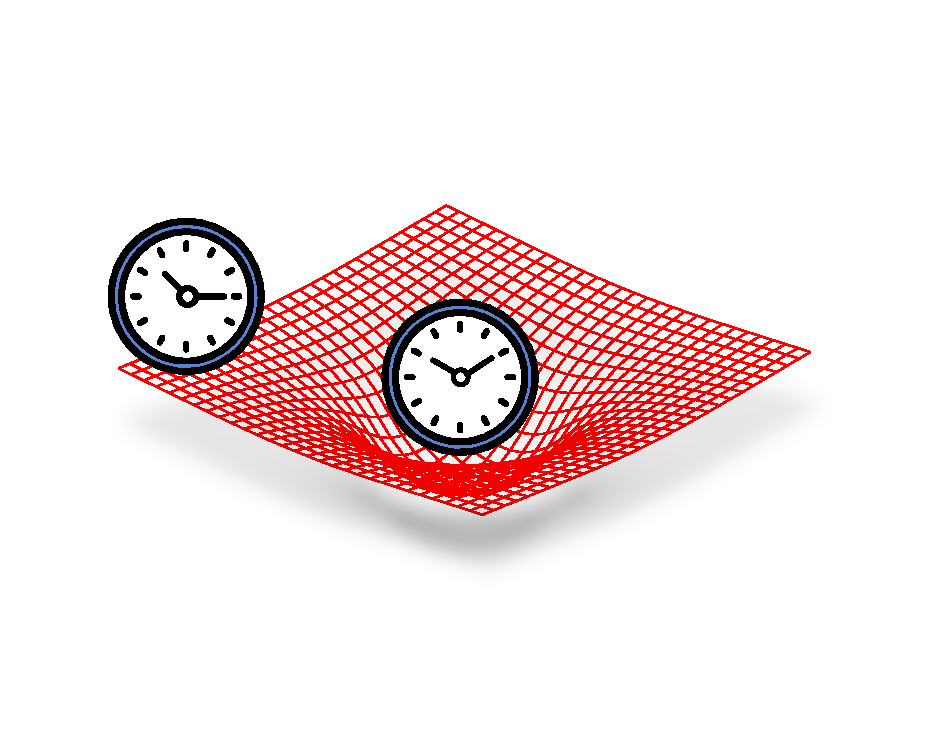
\includegraphics[trim=43bp 72bp 45bp 94bp,clip,width=0.88\linewidth,height=0.48\textheight,keepaspectratio]{../figs/pdf/en/fig-04-01.pdf}

% DOCX paragraph 400
\caption{\emph{El ritmo de avance de los relojes depende de la curvatura del
espaciotiempo y, por tanto, de su posición. Los que están en una región casi plana
del espaciotiempo avanzarán más deprisa que los que se encuentran en una zona muy
curvada.}}\label{fig:04-01}
\end{figure}

% DOCX paragraph 402
Volvamos al GPS. Lo dicho significa que los relojes de las estaciones terrestres,
donde la curvatura y la gravedad son mayores, acumularán un retraso de
aproximadamente 45 microsegundos (es decir, 45\,000 nanosegundos) por día, en
comparación con unos relojes idénticos colocados en los satélites que orbitan a
20\,000 kilómetros de la superficie terrestre, donde la curvatura y la gravedad
son menores. Esta diferencia de tiempo es mucho mayor que el máximo aceptable
para el correcto funcionamiento del GPS, que asciende a 40 nanosegundos por día.
Por tanto, si los relojes no se calibraran debidamente, el GPS proporcionaría
información totalmente incorrecta sobre nuestra posición.

% DOCX paragraph 403
Soy consciente de que todo esto puede sonar increíble o incluso absurdo; yo mismo
también tengo que hacer acopio de toda mi imaginación para aceptar un fenómeno tan
alejado de nuestra percepción\index{percepción} de la realidad. Pero,
afortunadamente para nosotros, lo que he expuesto ya no representa una consecuencia
abstrusa de una extraña teoría: es una predicción exacta que hoy en día ¡podemos
verificar experimentalmente! Pues sí, por más que suene a ciencia ficción, estamos
en condiciones de medir con precisión la diferencia en el ritmo del tictac de
relojes atómicos que sencillamente se colocan en pisos distintos de un edificio
corriente. La capacidad de llevar a cabo estas mediciones nos ha permitido confirmar
lo que Einstein predijo hace más de cien años: un reloj colocado en el primer piso
de un edificio y que, por lo tanto, se encuentra en un campo gravitatorio más
intenso, se retrasará con respecto a otro reloj idéntico situado en el segundo
piso, donde el campo es más débil. Como puedes imaginar, la diferencia es minúscula,
o sea que no intentes utilizar este argumento como excusa por haber llegado tarde
a una cita, explicando que tenías el reloj en un lugar con mucha curvatura del
espaciotiempo…

% DOCX paragraph 406
\section{En busca de una curvatura fuerte}\label{sec:04-search}

% DOCX paragraph 408
Volvamos ahora a la estimación de la curvatura que ofrece la ecuación
\eqref{eq:04-01}. Hemos establecido que la curvatura es casi igual a cero en nuestro
planeta, pero eso no impide que vayamos a «buscar» una curvatura más intensa en
nuestro barrio, digamos, en el sistema solar. Imaginemos que construimos un
dispositivo para medir la curvatura relativa y vamos saltando de planeta en planeta
para ver cómo varían los valores que medimos. ¿Qué descubriríamos? En primer lugar,
en el espacio interplanetario, donde hay muy poca materia, la curvatura es incluso
inferior a la de la Tierra, ¡luego el espaciotiempo es aún más plano por allí! La
curvatura solo sería perceptible al acercarnos a un planeta, pero de todos modos
los valores serían comparables a los que hemos visto para la Tierra. Si continuamos
nuestro viaje por el sistema solar, el dispositivo nos revelaría que el valor
máximo se alcanza en la superficie de nuestra estrella.

% DOCX paragraph 409
Para conocer la compacidad del
Sol\index{Sol!curvatura}\index{Sol!compacidad}\index{Sol!masa}\index{Sol!radio}, no hay
más que usar la ecuación \eqref{eq:04-02}, sustituyendo la masa y el radio de la
Tierra por los del Sol.

% DOCX paragraph 411
\begin{equation}\label{eq:04-03}
\begin{gathered}
\left(\textcolor{gray}{\frac{G}{c^{2}}}\frac{M_{\odot}}{R_{\odot}}\right)
\approx \left(\textcolor{gray}{\frac{G}{c^{2}}}\right)\frac{1{,}98\times 10^{30}\ \mathrm{kg}}{695\,000\ \mathrm{km}} \\
\approx 2\times 10^{-6}=0{,}000002
\end{gathered}
\end{equation}

% DOCX paragraph 412
% Equation number is generated with the preceding equation.

% DOCX paragraph 413
Como vemos, la compacidad del Sol\index{compacidad!Sol} es unas tres mil veces mayor
que la de la Tierra e igual a 0,000002, o dos partes por millón. De ahí resulta que
la curvatura del espaciotiempo en las proximidades de nuestra estrella es mayor que
la que experimentamos en nuestro planeta. Esto se debe a que la masa del Sol es
trescientas mil veces la de la Tierra, mientras que su radio solo es cien veces
mayor. En consecuencia, por lo que respecta al Sol, aunque el denominador del
cociente \emph{M/R} es mayor que para la Tierra, el numerador aumenta todavía más.
Y aun así, el valor de la curvatura es decepcionante de lo pequeño que es, tan
pequeño que, si tuviéramos que representarlo visualmente mediante la deformación de
una sábana, nos seguiría pareciendo plana incluso a aquellos de nosotros con mejor
vista.

% DOCX paragraph 414
Obviamente, si pudiéramos experimentar sus efectos directamente, la curvatura del
espaciotiempo cerca del Sol sería suficiente para producir variaciones perceptibles
en nuestra experiencia cotidiana. De hecho, el campo gravitatorio sería allí unas
28 veces mayor; por ejemplo, suponiendo que en la Tierra pesas unos 70 kilogramos,
la misma báscula, colocada hipotéticamente en la superficie del Sol, diría que
ahora tienes un «sobrepeso» considerable: ¡2000 kilos! En realidad, tu masa corporal
no habría sufrido ningún cambio; siempre podrías compensarlo yendo a pesarte a la
Luna\index{Luna}, donde descubrirías que has «perdido peso»: la báscula mostraría un
peso de solo 12 kilos. Análogamente, en la superficie del Sol, las diferencias
entre relojes situados en configuraciones similares a las del GPS serían del orden
de centésimas de segundo por día. Esta es una medida de tiempo de la que todos
tenemos una idea precisa: no hay más que pensar en cuánto la usamos en los deportes
de velocidad.

% DOCX paragraph 415
Calculando la compacidad tal como aparece en la ecuación \eqref{eq:04-01}, podemos
determinar fácilmente la curvatura relativa producida por cualquier objeto, lo cual
nos puede llevar a conclusiones sorprendentes e inesperadas. Tomemos, por ejemplo,
dos objetos muy distintos: una estrella como el Sol y una galaxia como nuestra
Vía Láctea\index{Vía Láctea}. Pues bien, el primero tiene una masa de un millón de
billones de billones de kilogramos (escrito de forma más simple,
10\textsuperscript{30} kilogramos): un valor que en astronomía se utiliza como unidad
de referencia y se denomina \emph{masa solar}. El segundo objeto tiene una masa de
aproximadamente un billón de masas solares, un número que corresponde más o menos
a la cantidad de estrellas que contiene. Esta información nos podría llevar a
concluir que la galaxia produce una curvatura proporcionalmente más intensa, dado
que la Vía Láctea\index{Vía Láctea} tiene una masa considerablemente mayor que la del
Sol. En realidad, no es el caso; basta con comparar la compacidad de los dos
objetos para darse cuenta de ello y comprender por qué. En particular, el radio del
Sol es del orden de 700\,000 kilómetros, mientras que el de nuestra galaxia es de
aproximadamente 16\,000 \emph{pársecs} (unos 53\,000 años luz, es decir,
10\textsuperscript{17} kilómetros).\textsuperscript{\hyperlink{note:04-03}{3}} Ahora,
si calculamos la compacidad\index{compacidad!Vía Láctea} \emph{M/R} de la Vía
Láctea\index{Vía Láctea}, nos daremos cuenta de que es comparable a la del Sol, o
sea, del orden de unas partes por millón (para ser precisos,
\emph{M/R} ≃1,80 × 10\textsuperscript{−6}). La razón es obvia: nuestra galaxia es
considerablemente más masiva, pero también mucho más extensa y diluida, de manera
que su compacidad no difiere mucho de la del Sol. En resumen, la curvatura producida
por estos dos objetos radicalmente distintos, y por tanto el radio de curvatura,
es casi la misma. Si estuviéramos a bordo de una nave espacial y nos acercáramos a
uno de los dos desde muy lejos (es decir, si nuestra nave actuara como lo que
técnicamente se denomina \emph{partícula de prueba}\index{partícula de prueba}),
experimentaríamos esencialmente el mismo campo gravitatorio y tendríamos que cambiar
nuestra trayectoria usando la misma cantidad de combustible.

% DOCX paragraph 416
Este ejemplo pretende servir de advertencia ante un error común al pensar en la
curvatura. En particular, cuando consideramos la curvatura producida por un objeto,
es engañoso centrarnos solo en su masa o su tamaño, ya que ambas cantidades nos
proporcionan únicamente una visión parcial. Por el contrario, el cociente entre
estas dos cantidades nos informa sobre cuánta masa \emph{M} está confinada en una
determinada región del espaciotiempo de tamaño \emph{R} para producir una curvatura
relativa proporcional a \emph{M/R}.

% DOCX paragraph 417
Por último, las estimaciones para la compacidad de la Tierra \eqref{eq:04-02} y del
Sol \eqref{eq:04-03} nos ayudarán a aprender una importante lección. En los dos
casos hay números extremadamente pequeños que corresponden a curvaturas muy
modestas y generan cambios igualmente pequeños en la dinámica de los objetos que
se mueven cerca de estos cuerpos. En otras palabras, la compacidad de la Tierra y
la del Sol nos dicen claramente que, a pesar de que el espaciotiempo es en
principio \emph{elástico}, es también muy \emph{rígido}. Básicamente, ¡la sábana de
nuestro ejemplo es bastante difícil de doblar!

% DOCX paragraph 418
Esta conclusión puede parecer desalentadora, ya que indicaría que la teoría de la
relatividad general de Einstein es fundamentalmente inútil. De hecho, la teoría se
centra en lo que ocurre cuando la curvatura es grande, pero todas nuestras
estimaciones nos dicen que es casi siempre cero o tan pequeña que puede
desestimarse, como ocurre con los experimentos en el CERN\index{CERN}.

% DOCX paragraph 421
\section{Una teoría que no le gustaba a nadie…}\label{sec:04-history}

% DOCX paragraph 423
Lo que se ha descrito hasta ahora, sobre todo la consideración de que el
espaciotiempo es muy difícil de doblar, nos ofrece una mejor comprensión del
desarrollo histórico de la relatividad general\index{relatividad general} y de
cómo fue recibida al principio dentro de la física moderna. Nos ayuda a apreciar
por qué esta teoría realmente no le gustaba a nadie salvo a unos pocos que la
comprendieron en detalle y a quienes les fascinó. Entre estos últimos figura el
ya mencionado sir Arthur Eddington\index{Eddington, sir Arthur}, apasionado defensor
de la teoría, quien la introdujo en la comunidad científica británica, una
comunidad que no tenía gran aprecio por las ideas de un científico alemán (no
olvidemos que se trata de los años de la Primera Guerra Mundial y el periodo
inmediatamente posterior).

% DOCX paragraph 424
Un gran número de científicos, incluso famosos, se opuso categóricamente a la
teoría de la relatividad general cuando se propuso. Esta actitud hacia las ideas
innovadoras de Einstein ---un rechazo que había comenzado mucho antes, con la
publicación de la teoría de la relatividad especial\index{relatividad especial}---
tenía diversas raíces, algunas de ellas muy profundas. Para empezar, los aspectos
matemáticos de la teoría eran tan complejos que muy pocas personas eran capaces de
seguirlos con detalle y captar sus consecuencias. Hay una anécdota al respecto que
ilumina la cuestión. Nos lleva a la presentación de Eddington\index{Eddington, sir Arthur}
de los resultados de las mediciones de la desviación de la luz durante el eclipse
solar\index{eclipse solar} total de 1919. Se dice que un periodista le preguntó a
Eddington\index{Eddington, sir Arthur} si era verdad que solamente tres personas en
todo el mundo comprendían la relatividad general\index{relatividad general}, a lo
cual él respondió, en tono de broma: «Ah, ¿sí? ¿Y quién sería el tercero?».

% DOCX paragraph 425
Esta actitud de rechazo hacia la nueva teoría de Einstein se debía en gran medida
al hecho de que proponía una visión radicalmente distinta de la gravedad: unas
consideraciones puramente matemáticas y geométricas (concretamente, la curvatura
del espaciotiempo) llegaban a explicar lo que se percibía como una interacción
puramente física.

% DOCX paragraph 426
Por añadidura, la protagonista de esta nueva teoría (la curvatura) siempre resulta
ser esencialmente igual a cero, al menos hasta donde era medible experimentalmente
en aquella época. No estaba pues claro qué repercusiones podría tener en la
práctica. Finalmente, para que el panorama desanimara más aún, la teoría daba lugar
a consecuencias aparentemente paradójicas o incluso absurdas, tales como la
dilatación del tiempo\index{dilatación del tiempo} o la contracción de las longitudes.

% DOCX paragraph 427
Muchas de estas objeciones, así como la actitud abiertamente hostil de numerosos
estudiosos, se superaron al confirmarse experimentalmente dos predicciones de la
teoría, a saber, la desviación de la luz y la precesión del
perihelio\index{perihelio} de Mercurio. Sin embargo, estos éxitos solo hicieron
cambiar la actitud «formal» de la comunidad científica hacia la relatividad
general, no su actitud en la práctica. Muchos físicos continuaban entonces (y
hasta cierto punto siguen en la actualidad) considerando que la teoría, si bien
no es incorrecta, es de escasa utilidad a efectos prácticos, aplicable a
condiciones físicas de curvatura muy diferentes de las que nos encontramos
habitualmente en la naturaleza.

% DOCX paragraph 428
Así pues, la relatividad general fue durante décadas una teoría de interés
principalmente para los matemáticos, quienes apreciaban su rica estructura y
elegancia geométrica. Por otra parte, los físicos seguían perplejos ante las
extrañas predicciones y algo intimidados por la complejidad de las ecuaciones, que
a menudo quedaban sin resolver, con excepción de unos pocos casos simples e
idealizados. Además, dadas las condiciones físicas para las que era relevante
(muy alejadas de las condiciones habituales en laboratorios y experimentos), la
relatividad general se aceptaba no tanto por ser correcta e importante, sino más
bien porque era fundamentalmente irrelevante. En otras palabras, la teoría de la
gravitación de Newton, aun siendo poco precisa, era más sencilla de usar y seguía
teniendo una precisión suficiente para ser la única teoría necesaria a efectos
prácticos.

% DOCX paragraph 429
Durante décadas, esta actitud escéptica condenó la relatividad general a un estado
de abandono, negándosele el desarrollo que merecía y que solo llegaría a conocer
muchos años más tarde. En efecto, una teoría recién formulada solo ofrece una idea
vaga de las implicaciones conceptuales y experimentales que puede llegar a tener
una vez plenamente desarrollada. Para explorar estas implicaciones de forma
detallada se requiere el esfuerzo colectivo de toda la comunidad científica, la
cual (a menudo sin un orden particular) se sumerge en los oscuros meandros de la
teoría para iluminar y revelar gradualmente sus diversos aspectos. Por desgracia,
nada de eso ocurrió en el caso de la teoría de la relatividad general. Entre 1916
(el año de su publicación) y principios de la década de 1960, fue prerrogativa de
un pequeño grupo de físicos y matemáticos interesados.

% DOCX paragraph 430
El punto de inflexión, que podría considerarse el «renacimiento» de la relatividad
general\index{relatividad general}, se dio cuando unas observaciones astronómicas
nuevas y sorprendentes (en particular, las obtenidas por satélites sensibles a la
radiación X\index{rayos X!radiación}\index{radiación!rayos X}) comenzaron a presentar
pruebas arrolladoras de la existencia de objetos celestes compactos cuya
fenomenología era imposible de explicar en el marco de la gravitación de Newton.
El innegable hecho de que existían objetos extremadamente compactos capaces de
liberar enormes cantidades de energía obligó a la comunidad científica a volver a
considerar las «extrañas soluciones» que la relatividad general había contemplado
casi cincuenta años antes.

% DOCX paragraph 431
La venganza de Einstein se hizo realidad cuando la propia naturaleza nos mostró
que, aunque el espaciotiempo es casi plano dentro del sistema solar, hay porciones
del universo donde esto no se cumple en absoluto. Además, las observaciones
astronómicas han revelado regiones del cosmos donde la naturaleza es capaz de
superar la tremenda rigidez del espaciotiempo, produciendo curvaturas elevadas que
pueden incluso llegar a ser extremas, como en el caso de los agujeros negros. En
condiciones semejantes, la relatividad general proporciona un marco matemático
adecuado y se convierte en la única teoría capaz de explicar, con enorme éxito,
el funcionamiento del mundo físico.

% DOCX paragraph 432
En los capítulos 5 y 6 estudiaremos dos de los ejemplos más llamativos de curvatura
extrema que puede producir la naturaleza, a saber, las estrellas de neutrones y
los agujeros negros. Pero antes nos espera una última consideración.

% DOCX paragraph 435
\section{Un experimento mental}\label{sec:04-experiment}

% DOCX paragraph 437
Antes de dar por terminado este capítulo, quiero invitarte a realizar lo que
Einstein llamaba un \emph{Gedankenexperiment}, es decir, un «experimento mental» que
se lleva a cabo usando únicamente la imaginación. Recordemos que, en general, la
finalidad de un experimento es determinar si un fenómeno se da tal como lo predice
la teoría, en condiciones muy precisas y reproducibles. Para llevar a cabo el
experimento, lo habitual es disponer de un laboratorio, un acelerador o
instrumentos tales como un satélite o un telescopio. En este sentido, un
experimento mental es algo decididamente anómalo, pues no requiere ningún tipo de
aparato experimental. En cambio, solo actúa nuestra mente, basándose en
consideraciones lógicas y físicas que nos permiten obtener unos resultados
«virtuales» que serían muy difíciles de alcanzar en un verdadero laboratorio. Por
decirlo de otra manera, un experimento mental es otra forma de hallar respuesta a
preguntas del estilo de «¿Qué sucedería si…?». Lo único que necesitamos para
llevarlo a la práctica es una buena dosis de imaginación y unos excelentes
conocimientos de física. Si tú te encargas del primer componente, yo te ayudaré
con el segundo para que entre los dos podamos llevar a cabo un experimento mental
para investigar los límites de la gravedad.

% DOCX paragraph 438
Comencemos pues con la ecuación \eqref{eq:04-01} para medir la compacidad de un
objeto. Hemos dicho que cuanto mayor es su valor, mayor es el grado relativo de
curvatura. Como la compacidad viene dada por el cociente entre la masa, \emph{M},
y el tamaño de un objeto, \emph{R}, podemos incrementar el valor de la razón
\emph{M/R} manteniendo constante el numerador y reduciendo gradualmente el
denominador. Desde el punto de vista de la física, en la práctica podemos tomar
un objeto, por ejemplo una estrella como el Sol, y comprimirlo progresivamente
para reducir su radio. Imaginemos una gigantesca prensa que «estruja» el Sol cada
vez más y reduce su radio según nuestros deseos; admito que aquí hace falta
bastante imaginación, ¡pero de eso se trata cuando hacemos experimentos mentales!
El resultado del proceso aparece esquemáticamente en la figura \ref{fig:04-02}.
Analicémoslo juntos.

% DOCX paragraph 439
En concreto, el panel de la izquierda muestra la curvatura del espaciotiempo cuando
hemos reducido el radio del Sol de sus 700\,000 kilómetros iniciales a unos 15, es
decir, el tamaño de una ciudad medianamente grande. Vemos que la compacidad
\emph{M/R} ha aumentado enormemente, del orden de dos millonésimas de la estimación
\eqref{eq:04-03} a 0,1, es decir, aproximadamente un
10\,\%\index{compacidad!estrella compacta}. Aquí podemos ver que la deformación de
la superficie es visible a simple vista, incluso sin ayudarnos de una escala de
grises (en los tres cuadros de la figura \ref{fig:04-02}, la «sábana» tiene una
longitud de 60 kilómetros). En particular, observa que la superficie apenas se
deforma en las zonas más alejadas del centro, es decir, en las esquinas, lo cual
indica que el espaciotiempo sigue siendo esencialmente
plano\index{espaciotiempo!plano (casi)}\index{espaciotiempo!curvado} en esas regiones.
En el centro, sin embargo, la curvatura es claramente visible y tiene la forma
suave de un cuenco.

% DOCX paragraph 442
\begin{figure}[htbp]
\centering
\[\begin{array}{@{}w{c}{0.2933\linewidth}@{}w{c}{0.2933\linewidth}@{}w{c}{0.2933\linewidth}@{}} R_{\odot}\cong15\ \mathrm{km} & R_{\odot}\cong7.5\ \mathrm{km} & R_{\odot}\cong5\ \mathrm{km}\end{array}\]

% DOCX paragraph 444
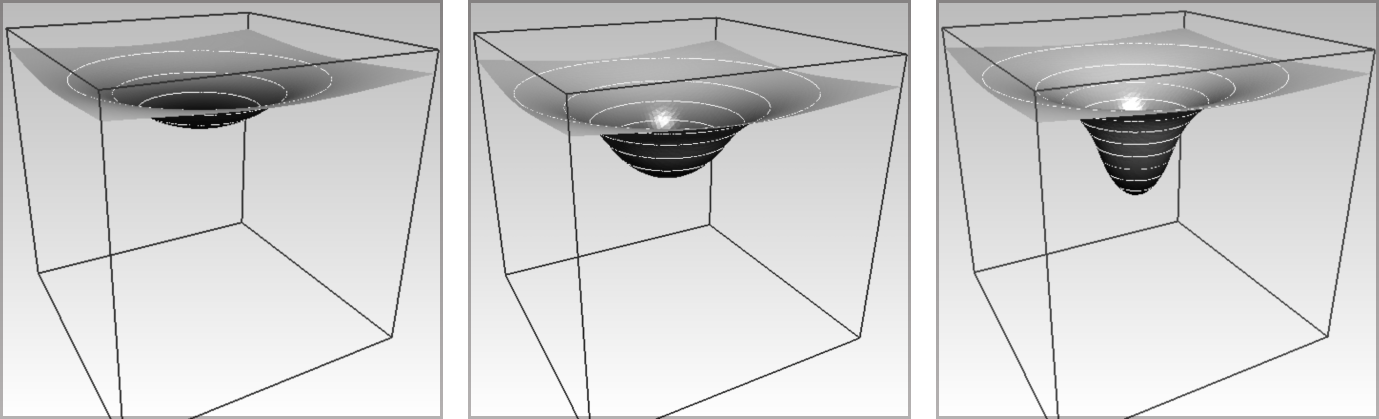
\includegraphics[width=0.88\linewidth,height=0.48\textheight,keepaspectratio]{../figs/pdf/en/fig-04-02.pdf}

% DOCX paragraph 446
\[\begin{array}{@{}w{c}{0.2933\linewidth}@{}w{c}{0.2933\linewidth}@{}w{c}{0.2933\linewidth}@{}} M/R\cong0.1 & M/R\cong0.2 & M/R\cong0.3\end{array}\]

% DOCX paragraph 447
\caption{\emph{Un experimento mental sobre la curvatura del espaciotiempo producida
por el Sol cuando su radio se reduce al valor indicado sobre cada cuadro, pero
su masa permanece constante. La compacidad relativa M/R se indica debajo de cada
imagen.}}\label{fig:04-02}
\end{figure}

% DOCX paragraph 449
El panel del centro de la figura \ref{fig:04-02}, por otra parte, nos muestra lo que
ocurriría si continuáramos con nuestro proceso y siguiéramos comprimiendo el Sol
hasta llegar a un radio de unos 7,5 kilómetros, la mitad del tamaño del cuadro
anterior. En este caso, la compacidad \emph{M/R} aumentaría a 0,2, es decir,
aproximadamente un 20\,\%. En esas condiciones, la curvatura llega a ser más
pronunciada aún y el «cuenco» que se forma en la sábana se hace mucho más profundo.
Podemos concluir nuestro experimento mental con el panel de la derecha en la
figura \ref{fig:04-02}, donde el Sol se ha comprimido hasta un radio de solo
5 kilómetros. Aquí la compacidad \emph{M/R} asciende a aproximadamente 0,3, un
30\,\%. La curvatura es muy pronunciada en estas condiciones y nuestra sábana,
que habíamos encontrado bastante rígida, se ha deformado enormemente. Lo que en
el panel izquierdo era un simple cuenco tiene ahora unas paredes muy empinadas;
se parece a lo que a menudo se llama «garganta\index{garganta}».

% DOCX paragraph 450
Es interesante comprobar que el grado de curvatura en el panel derecho de la
figura \ref{fig:04-02} es mucho más intenso que en el panel de la izquierda,
aunque al desplazarnos de uno al otro hemos reducido el tamaño de nuestra
estrella solo en una tercera parte. Esto se debe a que la curvatura depende de
manera no lineal del cociente entre masa y radio. En condiciones adecuadas,
modificar \emph{R} incluso muy ligeramente puede dar lugar a enormes variaciones
de la curvatura. Como es fácil imaginar si observamos la imagen de la derecha,
en condiciones de curvatura de este tipo pueden ocurrir nuevos fenómenos físicos
(que pueden medirse experimentalmente) muy diferentes de los que son habituales
en un espaciotiempo plano. En su debido momento exploraremos y explicaremos estos
fenómenos.

% DOCX paragraph 451
Quiero concluir este capítulo con unas pocas preguntas que espero que despierten
tu curiosidad. Hemos visto lo que le pasa a la curvatura del espaciotiempo
producida por el Sol cuando la estrella se reduce hasta un radio de tan solo cinco
kilómetros. Pero nos podríamos preguntar: «\emph{¿Hay un límite para la compresión
de un objeto como el Sol? En caso afirmativo, ¿cuál es ese límite?}». Y siguiendo
en esta línea: «\emph{Si el límite efectivamente existe, ¿se puede superar? ¿Y qué
ocurriría si fuera posible?}».

% DOCX paragraph 452
Hallaremos respuestas a estas preguntas en la siguiente etapa de nuestro viaje.
